% ---------------------------------------------------------------------------- 
% 
% $Description: Slides presentation using Beamer $
% 
% $Author: dloubach $
% $Release Date: September 28, 2015 $
% 
% This was first used in the Technical Discussions Seminar of our lab:
% Advanced Computing, Control & Embedded Systems Laboratory
% http://www.fem.unicamp.br/~acceslab
% 
% ------------------------------------------------------------------------- 

\documentclass[10pt, aspectratio=169]{beamer}
\usepackage{beamer-settings}   % customized presentation settings
\usepackage{multirow}
\usepackage{hyperref}

% presentation title
\title[COMP ITA]{CodeQL}
\subtitle[*]{Visão geral, conjugando teoria e prática.}

% author info
\author[Surname, Name]{
  \textbf{Marcelo Reis}\\
  \tiny{[Student] \\
    crereis@gmail.com} \\
}

% author affiliation
\institute[ITA]{
  Department of Computer Systems\\%
  Computer Science Division -- IEC\\%
  Aeronautics Institute of Technology -- ITA\\%

  \begin{figure}[h!]
    \centering
    
\includegraphics[scale=.17]{logo-ita-t}
  \end{figure}
}

\date{\tiny Today}

\pgfdeclareimage[width=0.110\textwidth]{university-logo}{figs/logo-ita-t}
\logo{\pgfuseimage{university-logo}}

\makeatletter
\makeatother


\begin{document}
\begin{frame}
  \titlepage
\end{frame}

\section[]{}
\begin{frame}
  \frametitle{Agenda}
  \tableofcontents
\end{frame}

\section{Motivation}
\begin{frame}
	\frametitle{Motivation}
	
	\begin{quotation}
		%Give your research context here
	\end{quotation}
	\begin{center}
		\begin{tabular}{c m{5cm}}
			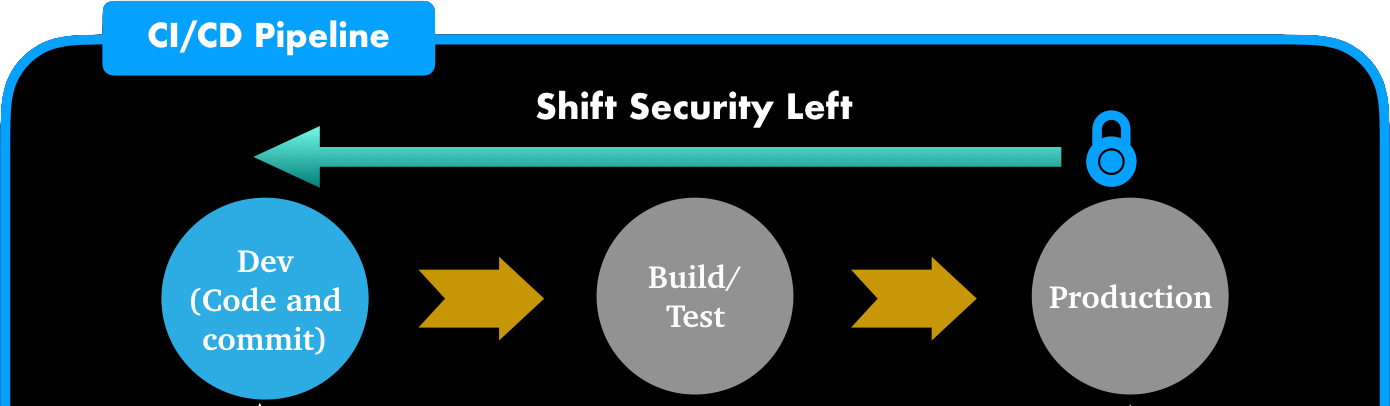
\includegraphics[scale=.15]{shifit_left_cuted} &\vspace{-1.5cm} \textbf{Como listar e navegar nos pontos do programa, cujo padrão sugere uma vulnerabilidade, antes da produção??}
			\\
		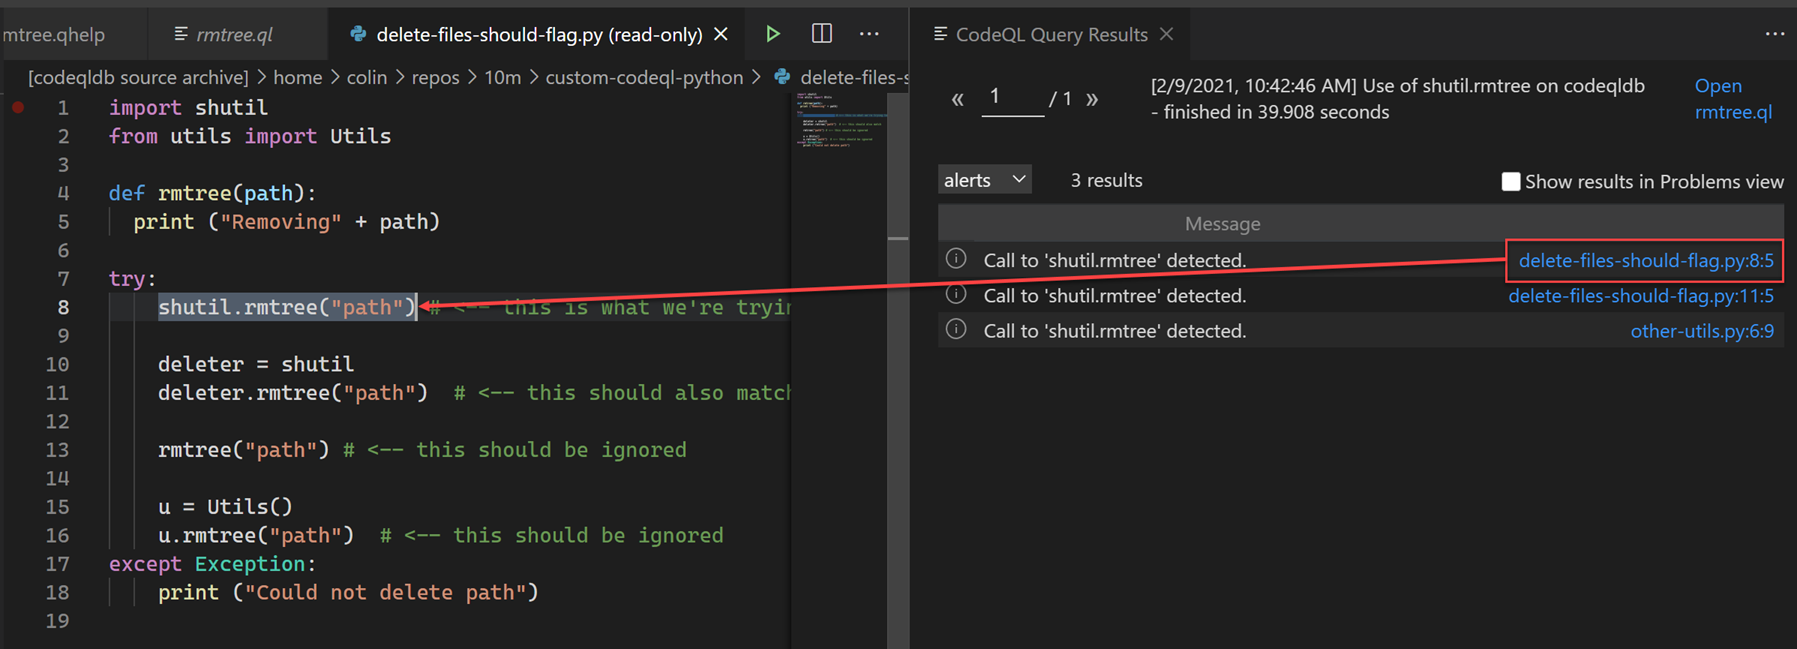
\includegraphics[scale=.12]{redirecionamento}&\vspace{-2.0cm} 
\includegraphics[scale=.12]{logoCodeQL}
		\end{tabular}
		
		%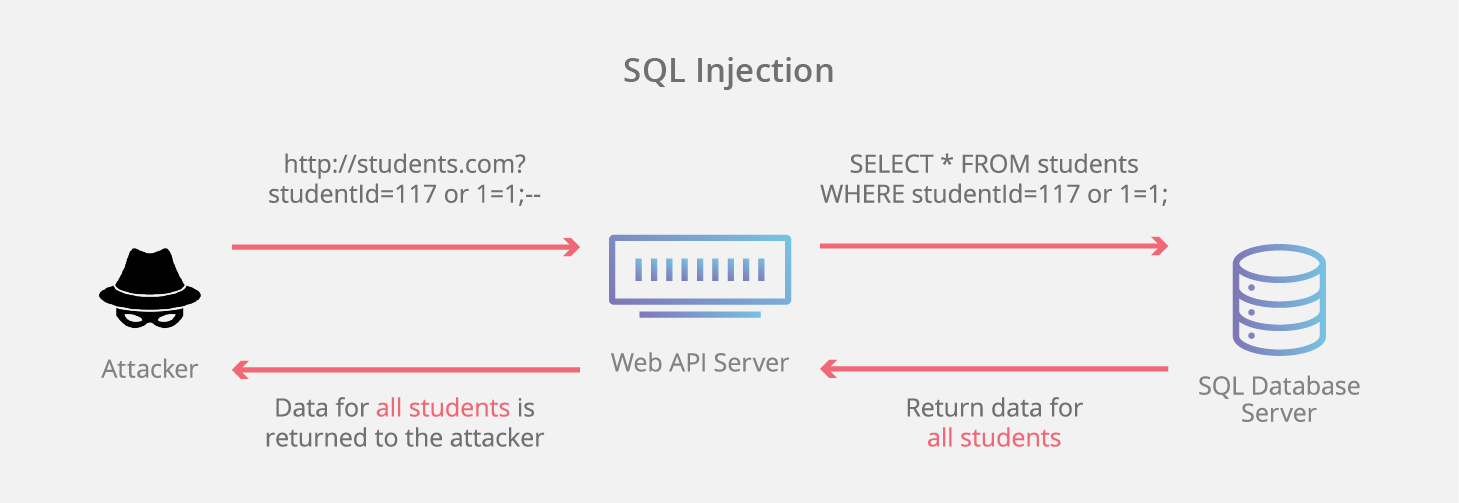
\includegraphics[scale=.32]{sql-injection-infographic}
		%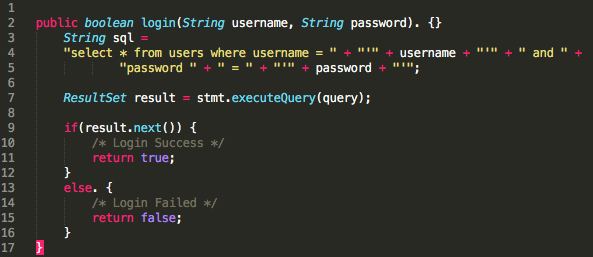
\includegraphics[scale=.32]{SQL-Injection-code}
	\end{center}
	
	
	
	%\begin{itemize}
	%\item \vfill Why this subject is relevant?
	%\item \vfill What are the main drawbacks of it?
	%\end{itemize}
	
	\vfill
	\vfill
	
	%Example of reference\footnote[frame]{\tiny\cite{Liu:1973aa}}
\end{frame}


\section{CodeQL}
\begin{frame}
  \frametitle{Definição e Princípios} 

  \begin{enumerate}
  \item \vfill Ferramenta de análise estática.
  \item \vfill Trata o código com dado
  \end{enumerate}
\begin{figure} 
	
	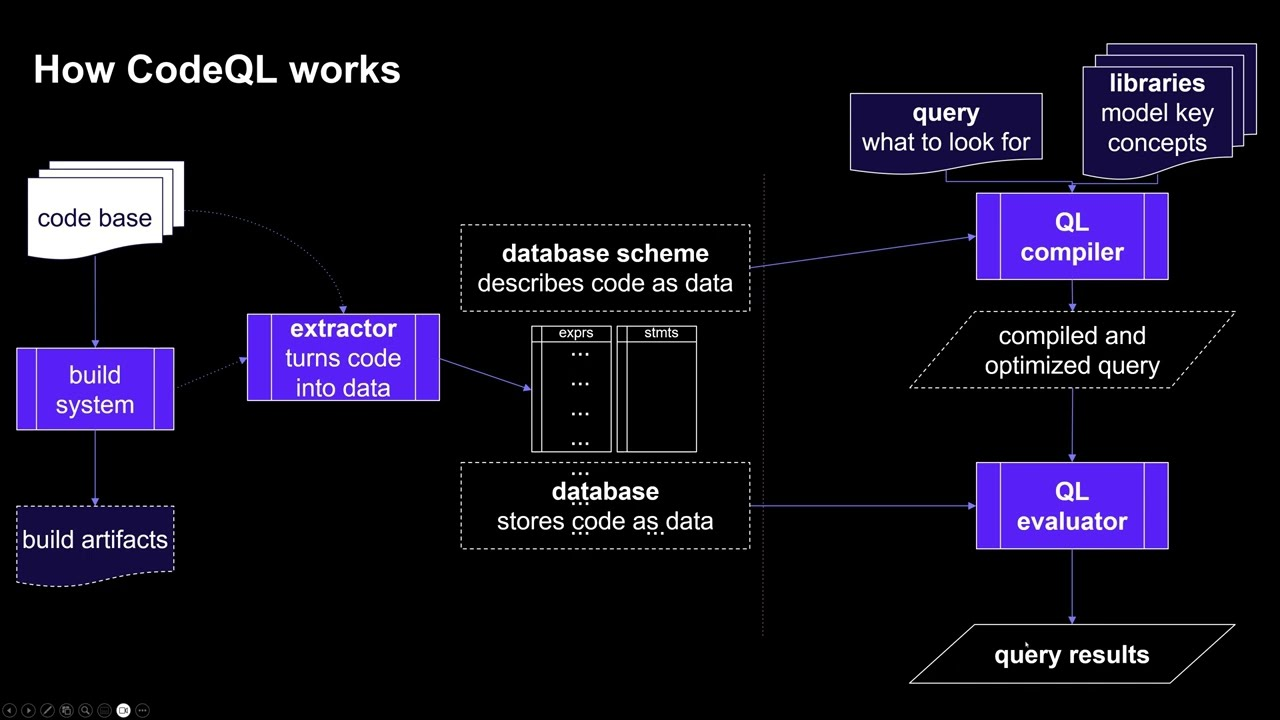
\includegraphics[scale=.25]{codeQLSchema}

\end{figure}
	
 


\end{frame}


\section{Exemplos Iniciais}
\begin{frame}
	\frametitle{Consultas Básicas}
	  \begin{itemize}
		\item  Analisar a ``Blocos Vazios''.
		\item  Retornos compostos por somas.
		\begin{itemize}
			\item return x+y;	
		\end{itemize}
		\item Comentários /*TODO.....
		\item Métodos com apenas um argumento
		
	\end{itemize}
	
	
	
\end{frame}


\section{SQL-Injection}
\begin{frame}
	\frametitle{SQL-Injection}
	
	\begin{quotation}
		%Give your research context here
	\end{quotation}
	\begin{center}
		\begin{tabular}{c c}
			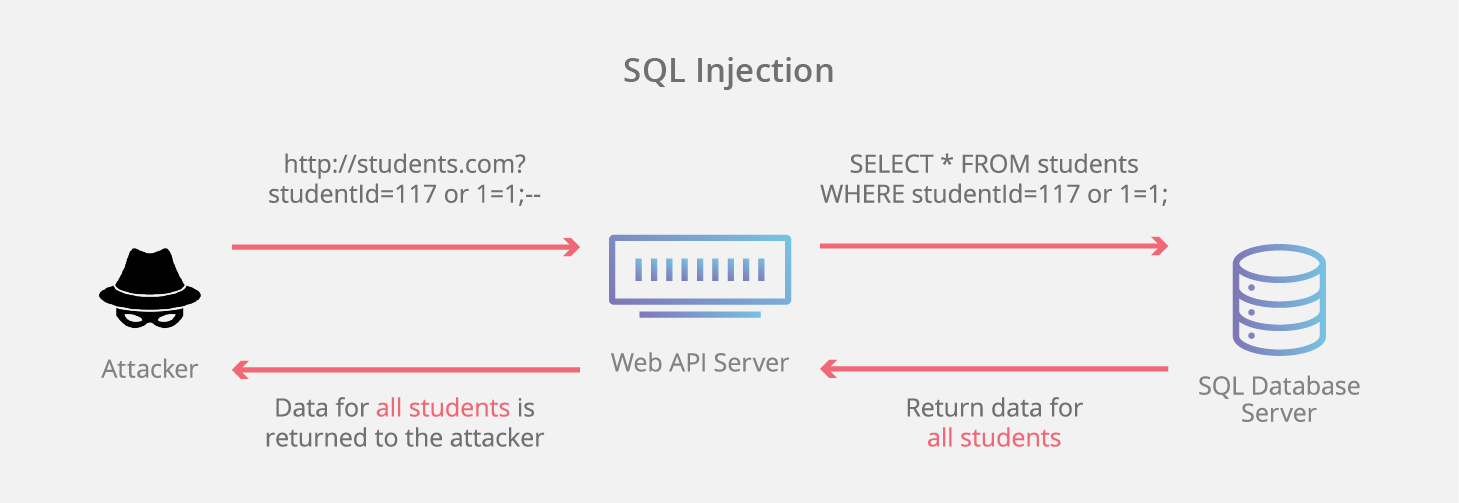
\includegraphics[scale=.30]{sql-injection-infographic} & \multirow{2}{4cm}{Como listar todos os pontos do programa em que consultas são passadas por meio de strings??!!}
			\\
			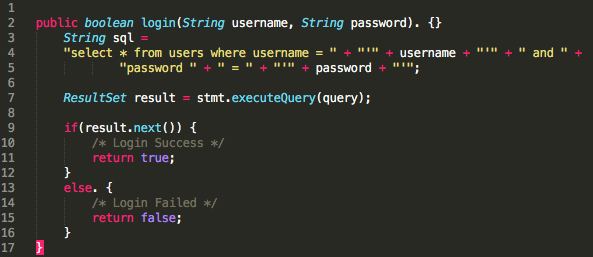
\includegraphics[scale=.30]{SQL-Injection-code}
		\end{tabular}
		
		%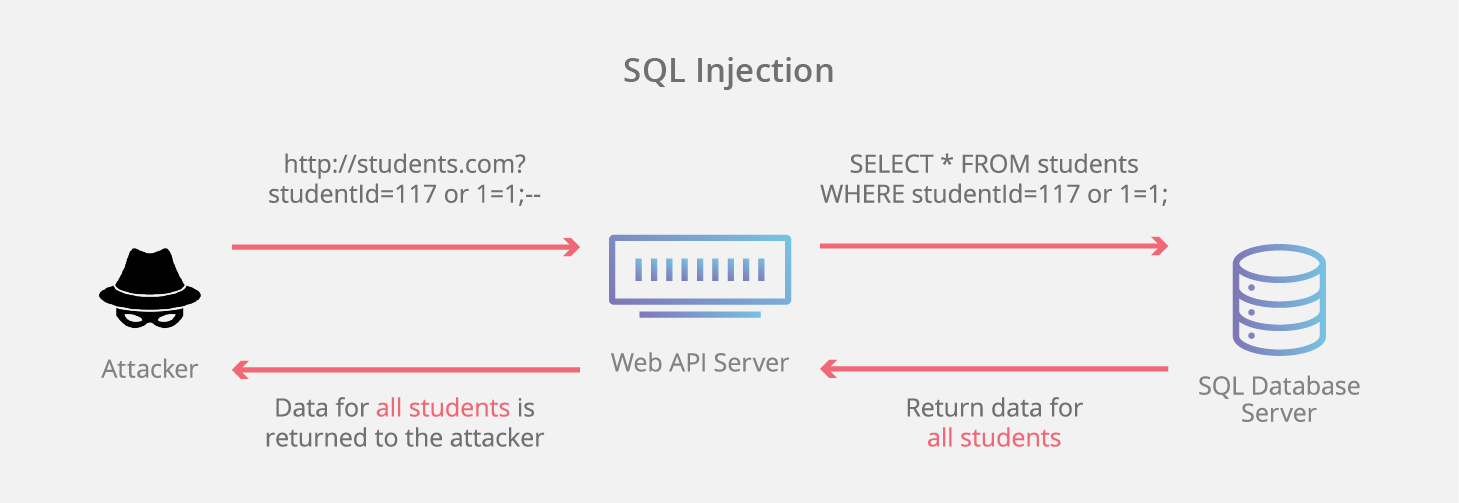
\includegraphics[scale=.32]{sql-injection-infographic}
		%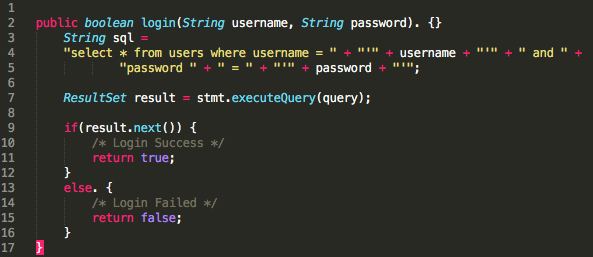
\includegraphics[scale=.32]{SQL-Injection-code}
	\end{center}
	
	
	
	%\begin{itemize}
	%\item \vfill Why this subject is relevant?
	%\item \vfill What are the main drawbacks of it?
	%\end{itemize}
	
	\vfill
	\vfill
	
	%Example of reference\footnote[frame]{\tiny\cite{Liu:1973aa}}
\end{frame}

\begin{frame}
	\frametitle{SQL-Injection}
	
	\begin{quotation}
		\Large{Melhor ainda....}
	\end{quotation}
	\begin{center}
		
		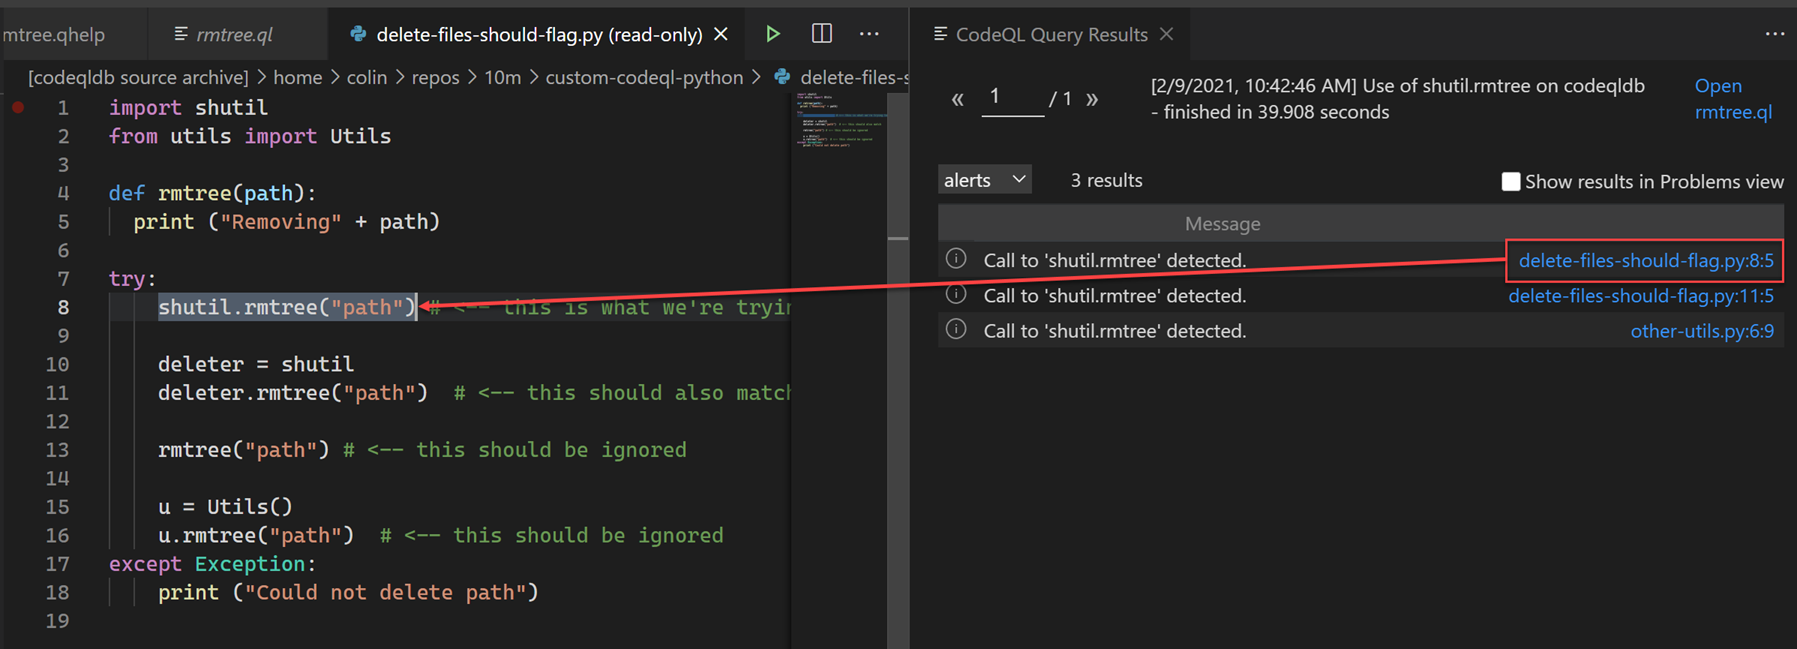
\includegraphics[scale=.22]{redirecionamento}
		%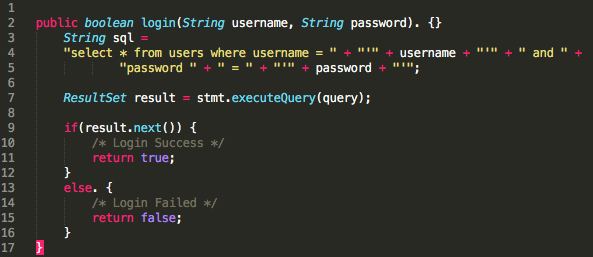
\includegraphics[scale=.32]{SQL-Injection-code}
	\end{center}
	
	
	
	%\begin{itemize}
	%\item \vfill Why this subject is relevant?
	%\item \vfill What are the main drawbacks of it?
	%\end{itemize}
	
	\vfill
	\vfill
	
	%Example of reference\footnote[frame]{\tiny\cite{Liu:1973aa}}
\end{frame}



\section{XSS}
\begin{frame}
	\frametitle{XSS}
	
	\begin{quotation}
		Execução de um trecho de código indesejado. 
	\end{quotation}
	\begin{center}
		\begin{tabular}{c c}
			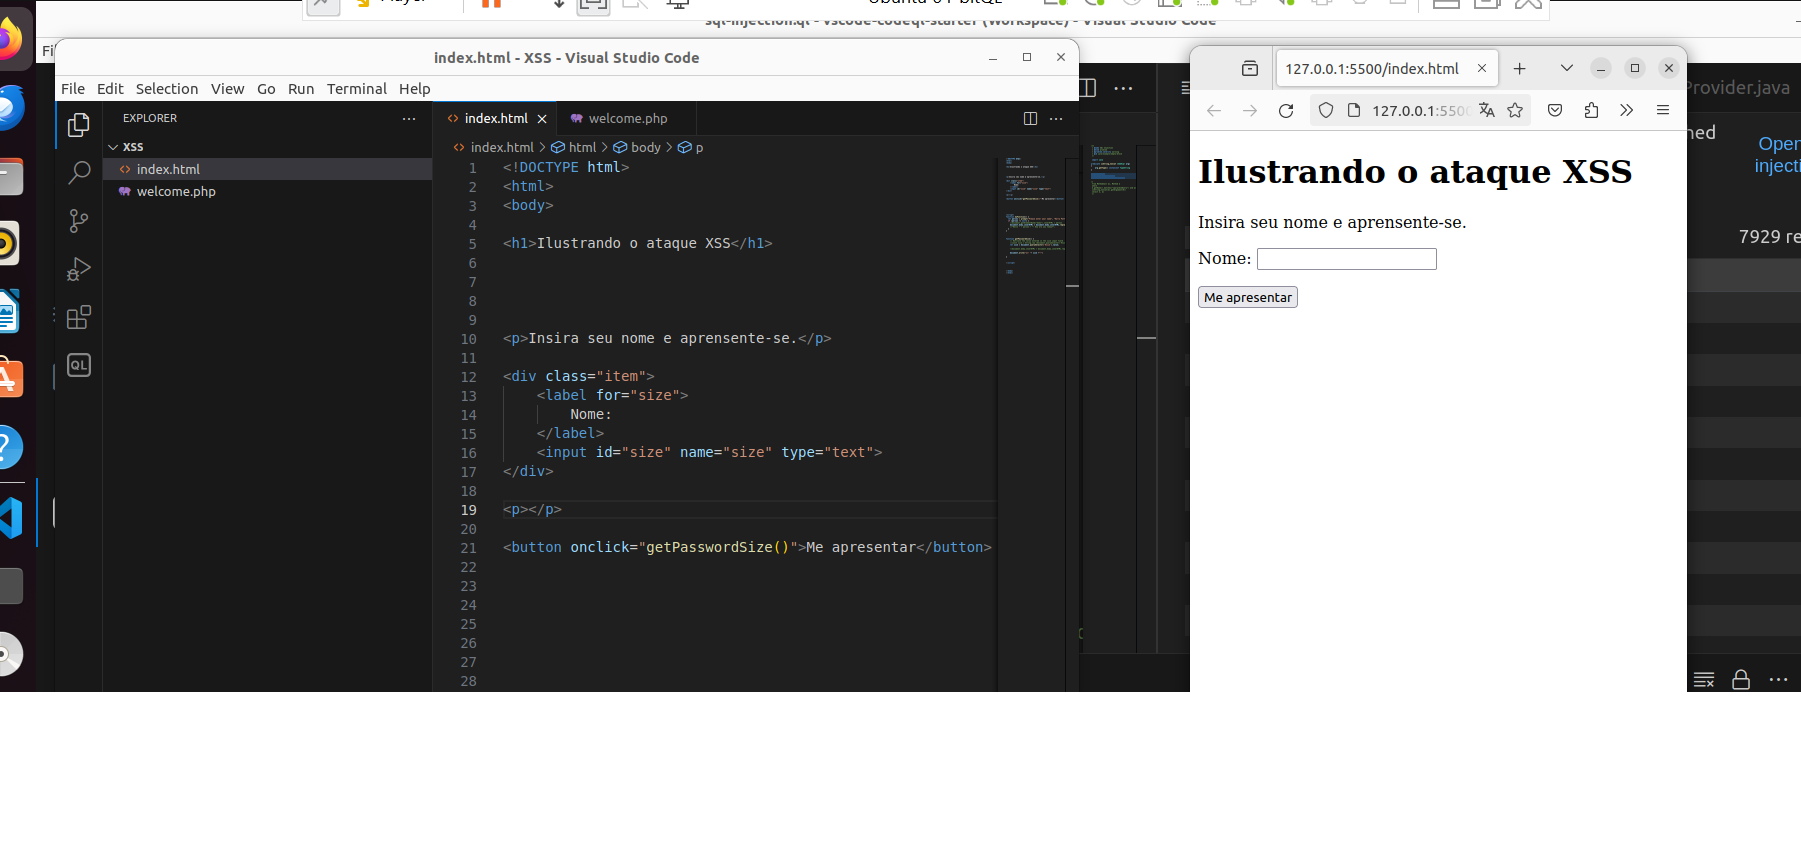
\includegraphics[scale=.30]{xss} & \multirow{2}{4cm}{Como listar todos os pontos do programa em que consultas são passadas por meio de strings??!!}
			\\
			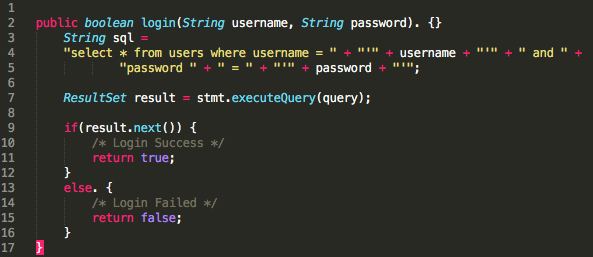
\includegraphics[scale=.30]{SQL-Injection-code}
		\end{tabular}
		
		%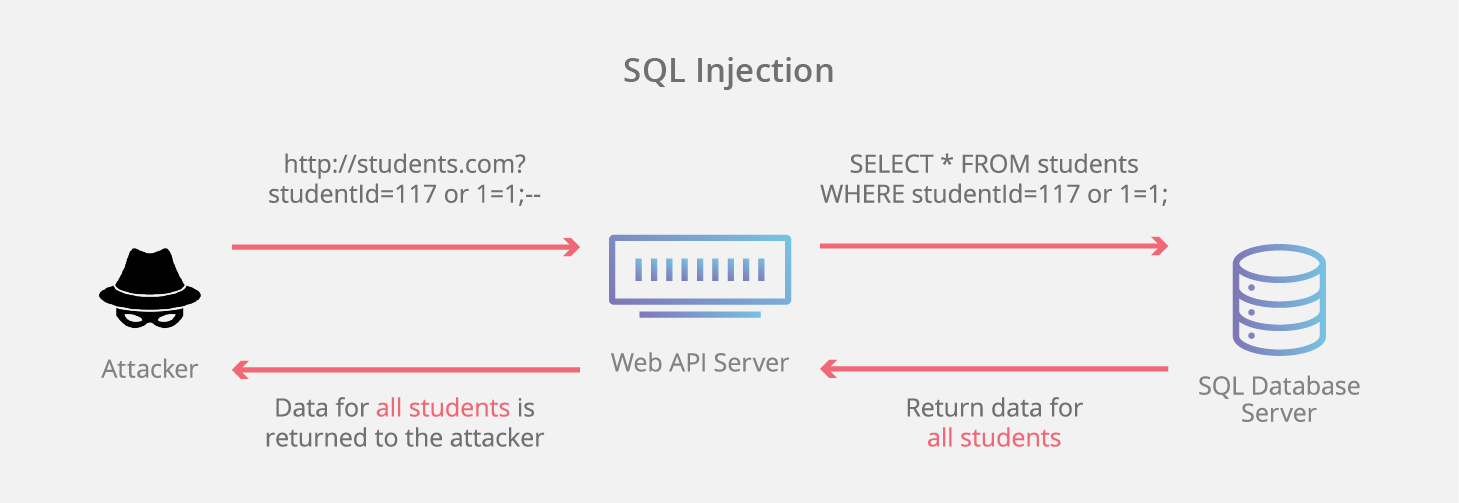
\includegraphics[scale=.32]{sql-injection-infographic}
		%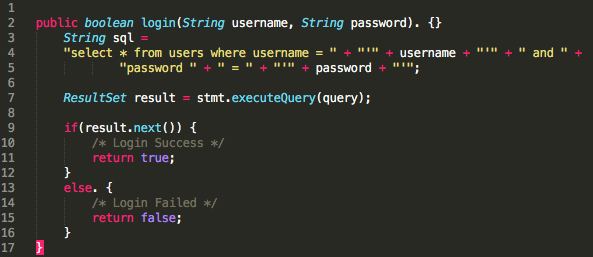
\includegraphics[scale=.32]{SQL-Injection-code}
	\end{center}
	
	
	
	%\begin{itemize}
	%\item \vfill Why this subject is relevant?
	%\item \vfill What are the main drawbacks of it?
	%\end{itemize}
	
	\vfill
	\vfill
	
	%Example of reference\footnote[frame]{\tiny\cite{Liu:1973aa}}
\end{frame}


\section{Conclusion}
\begin{frame}
  \frametitle{Conclusion}
  	\begin{quotation}
  	Bem-vindo ao vasto mundo do codeQL. 
  \end{quotation}
  
 \end{frame}


\section{Questions \& Answers}
\begin{frame}
  \frametitle{Questions \& Answers}

  \begin{quotation}
  \end{quotation}
  \flushright

\end{frame}


\end{document}

%%% Local Variables:
%%% mode: latex
%%% TeX-master: t
%%% End:
